\documentclass[12pt]{article}
\usepackage{graphicx, geometry, hyperref} % Required for inserting images
\usepackage{physics,caption, amsmath, amsfonts, tikz, minted}
\usepackage{scalerel, cases, multirow, multicol}
\usepackage{tabularx}
\graphicspath{{images/}}
\hypersetup{colorlinks=true,citecolor=black,linkcolor=black,urlcolor=black}
\geometry{
a4paper,
total={170mm,257mm},
left=20mm,
top=20mm,
}
\usepackage[table]{xcolor}
\usepackage{eulervm}
\usepackage{booktabs}


%-------------new commands----------------------
\newcommand{\bc}[1]{{\color{blue}{#1}}}
\newcommand{\red}[1]{{\color{red}{#1}}}

\begin{document}

\begin{center}
    \Large \bfseries{Weekly Report}
\end{center}

\begin{center}
    \Large \bfseries{CS3500: Operating Systems}
\end{center}


\begin{center}
    \Large \bfseries{Visualisation Tool for Process Scheduling}
\end{center}
\begin{center}
    \vspace{1.2cm}
    
\includegraphics[width=5cm]{logos and images/IIT_Madras_Logo.svg.png}

    \textbf{Computer Science and Engineering}
    \vspace{0.3cm}

    \textbf{Indian Institute of Technology  Madras}
    \vspace{0.3cm}

    \textbf{Jul - Nov 2024}
    \vspace{1.2cm}

    \noindent \textbf{Under the supervision}
    \vspace{0.2cm}

    \noindent \textbf{of}
    \vspace{0.2cm}

    \noindent\textbf{Prof. Janakiram D}
     \vspace{0.2cm}

    \noindent \textbf{submitted by}
    \vspace{0.3cm}

    \noindent \textbf{Team 8}
    \begin{multicols}{2}
        \begin{itemize}
            \item Anjali Samudrala (CS22B046)
            \item Chaitanya Sai Teja G (CS22B036)
            \item Jwala Likitha Reddy M (CS22B078)
            \item Karthikeya P (CS22B026)
            \item Naveen Koushik Reddy E (CS22B006)
            \item Navya Sree B (CS22B045)
            \item Rushi Babu G (CS22B040)
            \item Sravya Rangu (CS22B044)
            \item Yashwanth Sai P (CS22B002)
            \item Yaswanth Sai V (CS22B043)
        \end{itemize}
    \end{multicols}
    \vspace{0.5cm}

\end{center}
\clearpage
\tableofcontents
\clearpage
\listoffigures
\clearpage

\section{Design Choices}
\subsection{Frontend}
We choose to use ReactJS for the frontend of our project. ReactJS is a JavaScript library that is used to build user interfaces. It is maintained by Facebook and a community of individual developers and companies. ReactJS is used for handling the view layer for web and mobile apps. ReactJS allows us to create reusable UI components. It is currently one of the most popular JavaScript libraries and has a strong foundation and large community behind it. We chose ReactJS because it is easy to learn and use, and it allows us to create a dynamic and interactive user interface.

\subsection{Backend}
We choose to use Flask for the backend of our project. Flask is a micro web framework written in Python. It is lightweight and easy to use. Flask is designed to make getting started quick and easy, with the ability to scale up to complex applications. We chose Flask because it is easy to learn and use, and it allows us to create a RESTful API for our project. Flask is also easy to deploy and maintain, which makes it a good choice for our project.

\subsection{Communication between Frontend and Backend}
We are using the socket framework to establish communication between the frontend and the backend. The socket framework allows us to establish a bidirectional communication channel between the client and the server. This allows us to send and receive data in real-time, which is important for our project. We are using the socket.io library for the frontend and the Flask-SocketIO library for the backend. These libraries make it easy to establish a socket connection between the client and the server and send and receive data in real-time.

\section{Plots}
\subsection{CPU usage by Process}
\begin{figure}[H]
    \centering
    \begin{minipage}{0.45\textwidth}
        \centering
        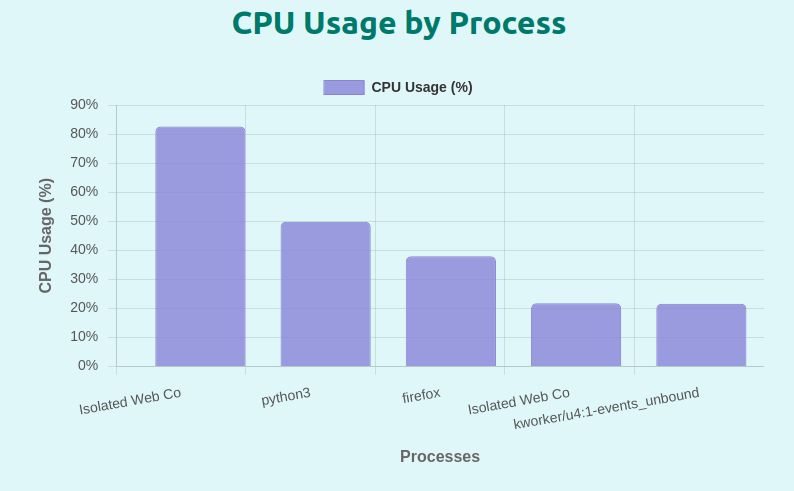
\includegraphics[width=\textwidth]{logos and images/PLOT1_1.png}
    \end{minipage}
    \hfill
    \begin{minipage}{0.45\textwidth}
        \centering
        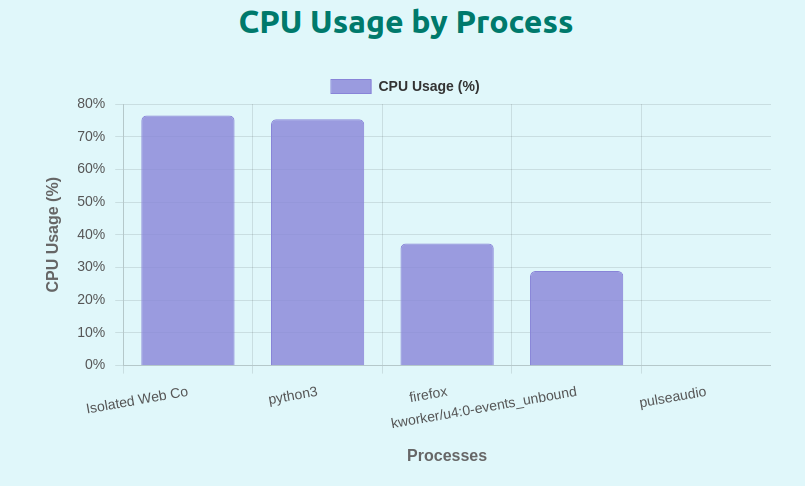
\includegraphics[width=\textwidth]{logos and images/PLOT1_2.png}
    \end{minipage}
    \caption{Top 5 High-Load Processes at different time instances}
\end{figure}
This plot shows the top 5 high-load processes in the system. The x-axis represents the process ID, and the y-axis represents the \% CPU load of the process. The plot shows the CPU load at two different instances of the time. The plot is updated in real-time, so the user can see the CPU load of the top 5 high-load processes as it changes over time.

\subsection{CPU-Usage Stream}
\begin{figure}[H]
    \centering
    \begin{minipage}{0.45\textwidth}
        \centering
        \includegraphics[width=\textwidth]{logos and images/PLOT2_1.png}
    \end{minipage}
    \hfill
    \begin{minipage}{0.45\textwidth}
        \centering
        \includegraphics[width=\textwidth]{logos and images/PLOT2_2.png}
    \end{minipage}
    \caption{Snapshots of the activity tracker at two different instances}
\end{figure}

This plot displays a real-time visualization of the activity of processes over multiple snapshots, represented by a stacked bar chart. Each bar in the chart corresponds to a snapshot of processes, showing whether each process (identified by its PID) was active at that moment. The chart uses distinct colors for each process, making it easy to track process activity over time. The x-axis represents different snapshots, while the y-axis shows the number of processes. This visualization helps in monitoring the system’s process behavior, observing trends, and identifying active or idle processes in real time.




\subsubsection{Frontend Implementation}
\begin{itemize}
    \item PLOT1
    \begin{minted}{javascript}
    import React from 'react';
    import {BarChart, Bar, XAxis, YAxis, CartesianGrid, Tooltip, Legend} from 
        'recharts';
    import '../App.css';

    function Plot1({ processes }) {
    return (
        <div className="processes">
            <h2>CPU Usage</h2>
            <BarChart
            width={600}
            height={300}
            data={processes}
            margin={{
                top: 5, right: 30, left: 20, bottom: 5,
            }}
            >
            <CartesianGrid strokeDasharray="3 3" />
            <XAxis dataKey="name" />
            <YAxis />
            <Tooltip />
            <Legend />
            <Bar dataKey="cpu_percent" fill="#8884d8" />
            </BarChart>
        </div>
    )
    }

    export default Plot1;
\end{minted}

This frontend implementation for visualizing CPU usage utilizes the \textbf{Recharts} library to create an interactive bar chart. The component \texttt{Plot1} is responsible for rendering the chart. It takes a \texttt{processes} prop, which contains the updated process data, and displays CPU usage for each process.



\item PLOT2
\begin{minted}{javascript}
import React, { useEffect, useState } from "react";
import { Bar } from "react-chartjs-2";
import "chart.js/auto";
import ChartDataLabels from "chartjs-plugin-datalabels"; 


function Plot2({ processes }) {
  const [queue, setQueue] = useState([]);
  const [colorMap, setColorMap] = useState(new Map());

  const generateDistinctColor = (pid) => {
    const hash = pid * 2654435761 % 360; 
    return `hsl(${hash}, 70%, 50%)`;
  };

  useEffect(() => {
    if (processes.length > 0) {
      setQueue((prevQueue) => {
        const newQueue = [...prevQueue, processes];
        if (newQueue.length > 6) newQueue.shift();
        return newQueue;
      });

      setColorMap((prevColorMap) => {
        const updatedMap = new Map(prevColorMap);
        processes.forEach((process) => {
          if (!updatedMap.has(process.pid)) {
            updatedMap.set(process.pid, generateDistinctColor(process.pid));
          }
        });
        return updatedMap;
      });
    }
  }, [processes]);

  const chartData = {
    labels: queue.map((_, index) => `Snapshot ${index}`),
    datasets: Array.from(colorMap.keys()).map((pid) => ({
      label: `PID: ${pid}`,
      data: queue.map((snapshot) =>
        snapshot.find((p) => p.pid === pid) ? 1 : 0
      ),
      backgroundColor: colorMap.get(pid),
      borderWidth: 1,
      datalabels: {
        display: true,
        color: "white", 
        align: "center",
      },
    })),
  };

  const chartOptions = {
    responsive: true,
    maintainAspectRatio: false,
    plugins: {
      datalabels: {
        color: "#fff",
        formatter: (value, context) => {
        
          const datasetIndex = context.datasetIndex;
          const pid = chartData.datasets[datasetIndex].label.split(": ")[1];
          return value > 0 ? `PID: ${pid}` : "";
        },
        anchor: "center",
        align: "center",
        clip: true,
      },
      legend: {
        display: false, 
      },
    },
    scales: {
      x: {
        stacked: true,
        categoryPercentage: 0.01, 
      },
      y: {
        beginAtZero: true,
        stacked: true,
        title: {
          display: true,
          text: "Processes",
        },
      },
    },
  };

  return (
    <div className="processes" style={{ height: "400px" }}>
      <Bar data={chartData} options={chartOptions} plugins={[ChartDataLabels]} />
    </div>
  );
}

export default Plot2;

\end{minted}

\begin{itemize}
    \item This frontend implementation for \texttt{Plot2} involves the creation of a stacked bar chart to visualize snapshots of processes over time using the \textbf{Chart.js} library. The chart is rendered inside the \texttt{Plot2} React component, which maintains two states: \texttt{queue} (an array storing the most recent process snapshots) and \texttt{colorMap} (a map associating each process PID with a unique color). The component dynamically updates these states based on the incoming process data, ensuring that the chart displays up to six most recent snapshots. Each process is represented as a colored bar, and the chart is designed to show the active state of each process in each snapshot.\\
    \item The chart is customized to be stacked, with each process PID having its own bar in each snapshot. The \texttt{ChartDataLabels} plugin is used to display the process PID inside the bars for active processes, helping users identify processes easily. The chart scales automatically and is responsive to fit various screen sizes. The x-axis represents the snapshots, while the y-axis displays the number of processes, with the bars stacked to show process activity in each snapshot.
\end{itemize}


\end{itemize}

\subsubsection{Backend Implementation}
\begin{itemize}
    \item \texttt{MONITOR\_CPU()}
    \begin{minted}{python}
def monitor_cpu():
    global process_data, killed_processes
    while True:
        update_process_data()
        socketio.emit('cpu_data', process_data) 
        time.sleep(SLEEP_INTERVAL)
        process_data = [proc for proc in process_data if proc['pid'] not in 
                         killed_processes]
        killed_processes.clear()  
\end{minted}

\begin{itemize}
    \item \texttt{PURPOSE:}
    \begin{itemize}
        \item The function continuously monitors the CPU usage of processes, updates the global list of top CPU-consuming processes (\texttt{process\_data}), and emits this data to connected clients via a \texttt{Socket.IO} event. The monitoring and emission occur repeatedly with a delay defined by \texttt{SLEEP\_INTERVAL}.
    \end{itemize}
    
   \item \texttt{KEY\_VARIABLES:}
   \begin{itemize}
    \item \textbf{\texttt{process\_data}}: The global list of processes with their CPU usage information, which is updated by the \texttt{update\_process\_data} function.
    \item \textbf{\texttt{SLEEP\_INTERVAL}}: The interval (in seconds) between consecutive updates and emissions.
\end{itemize}
   \item \texttt{CODE\_ANALYSIS:}
   \begin{itemize}
       \item Continuous Monitoring:
       \begin{itemize}
    \item Runs an infinite loop to perform monitoring tasks without interruption.
\end{itemize}

\item {Update Process Data}
\begin{itemize}
    \item Calls the \texttt{update\_process\_data} function to refresh the global process information with the latest CPU usage and status.
\end{itemize}

\item {Emit Data to Clients}
\begin{itemize}
    \item Sends the updated \texttt{process\_data} to all connected clients using a \texttt{Socket.IO} event named \texttt{cpu\_data}.
    \item Ensures real-time communication of CPU usage data to the client-side application.
\end{itemize}

\item {Sleep Interval}
\begin{itemize}
    \item Introduces a delay between consecutive iterations to prevent overloading the system and allow sufficient time for data collection.
\end{itemize}
   \end{itemize}


\end{itemize}

\item \texttt{UPDATE\_PROCESS\_DATA()}
    \begin{minted}{python}
 def update_process_data():
    global process_data, killed_processes
    
    processes = []
    current_pids = set()

    for proc in psutil.process_iter(['pid', 'name', 'cpu_percent','create_time']):
        try:
            current_pids.add(proc.info['pid'])
            processes.append({
                'pid': proc.info['pid'],
                'name': proc.info['name'],
                'cpu_percent': proc.info['cpu_percent'],
                'create_time': datetime.datetime.fromtimestamp(
                proc.info['create_time']).strftime('%Y-%m-%d %H:%M:%S'),
            })
        except (psutil.NoSuchProcess, psutil.AccessDenied):
            continue

    for proc in processes:
        pid = proc['pid']
        
        existing_proc = next((p for p in process_data if p['pid'] == pid), None)
        if existing_proc:
            existing_proc['cpu_percent'] = proc['cpu_percent']
        else:
            process_data.append({
                'pid': pid,
                'name': proc['name'],
                'cpu_percent': proc['cpu_percent'],
                'create_time': proc['create_time'],
            })

    for proc in process_data:
        if proc['pid'] not in current_pids:
            proc['cpu_percent'] = 0
            killed_processes.add(proc['pid'])

    process_data = sorted(process_data, key=lambda x: x['cpu_percent'],
                  reverse=True)[:NUM_PROCESSES]
\end{minted}

 \begin{itemize}
    \item \texttt{PURPOSE:}
    \\
       The function maintains and updates a global list of processes (\texttt{process\_data}) by:
\begin{itemize}
    \item Collecting information about currently running processes.
    \item Updating CPU usage for active processes.
    \item Marking terminated processes as inactive.
    \item Limiting the list to the top \texttt{NUM\_PROCESSES} by CPU usage.
\end{itemize}
    
   \item \texttt{KEY\_VARIABLES:}
   \begin{itemize}
    \item \texttt{process\_data}: A global list containing information about processes, including PID, name, CPU usage, and creation time.
    \item \texttt{killed\_processes}: A global set that stores the PIDs of processes marked as terminated.
    \item \texttt{processes}: A local list temporarily storing process information retrieved during the current function execution.
    \item \texttt{current\_pids}: A local set of PIDs for all currently running processes.
\end{itemize}
   \item \texttt{CODE\_ANALYSIS:}
   \begin{itemize}
       \item {Retrieve Process Information}
\begin{itemize}
    \item Iterates through all processes using \texttt{psutil.process\_iter} with attributes \texttt{pid}, \texttt{name}, \texttt{cpu\_percent}, and \texttt{create\_time}.
    \item Safely handles exceptions for processes that no longer exist or are inaccessible.
    \item Collects CPU usage and timestamps in a standardized format (\texttt{YYYY-MM-DD HH:MM:SS}).
\end{itemize}

    \item {Update Process Data}
\begin{itemize}
    \item For each process, checks if it already exists in \texttt{process\_data}.
    \item Updates CPU usage if the process is found, or adds a new entry if it is not.
\end{itemize}
 
\item {Mark Terminated Processes}
\begin{itemize}
    \item Processes that no longer appear in the current set of PIDs are marked as inactive by setting their \texttt{cpu\_percent} to 0.
    \item Their PIDs are added to the \texttt{killed\_processes} set.
\end{itemize}

\item {Sort and Limit Process List}
\begin{itemize}
    \item Sorts \texttt{process\_data} by CPU usage in descending order.
    \item Trims the list to the top \texttt{NUM\_PROCESSES} by CPU usage.
\end{itemize}
\end{itemize}

\end{itemize}

\end{itemize}



\subsubsection{Data used for the plot}
\begin{itemize}
    \item For PLOT1
    \begin{itemize}
        \item \texttt{name}: The name of the process.
        \item \texttt{cpu\_percent}: The CPU usage percentage of the process.
    \end{itemize}
    \item For PLOT2
    \begin{itemize}
        \item \texttt{PID (Process ID)}: A unique identifier for each running process.
        \item \texttt{Snapshot Information}: A boolean or binary indicator (1 or 0) that represents whether a process was active in that particular snapshot.
        \item \texttt{Timestamp}: Used implicitly by the order of snapshots to track when each snapshot occurred.
    \end{itemize}

\end{itemize}
\subsubsection{Challenges faced}
\begin{itemize}
    \item For PLOT1
    \begin{itemize}
      
        \item \texttt{Handling Inaccessible or Terminated Processes}: Ensuring that terminated or no longer accessible processes are excluded or marked as inactive when using \texttt{psutil} to avoid errors.
        
        \item \texttt{Accurate Data Synchronization}: Consistently updating the process data across the backend to reflect real-time changes in process states and CPU usage.
        
        \item \texttt{Real-Time Updates Without Lag}: Ensuring that the frontend receives and displays real-time data updates without causing performance bottlenecks or delays, especially when the number of processes increases.
        
        \item \texttt{Responsive Chart Layout}: Adapting the chart to different screen sizes and resolutions while maintaining clarity and usability.

    \end{itemize}
    \item For PLOT2
    \begin{itemize}
        \item \texttt{Color Management}: Ensuring each process had a unique, consistent color across snapshots required a deterministic color generation function.
        
        \item \texttt{Performance Optimization}: Efficient management of the dynamic process snapshot queue was needed to avoid performance issues, especially as the number of processes increased.
        
        \item \texttt{Real-Time Data Synchronization}: Keeping process data updated in real-time while ensuring the frontend displayed the latest snapshots was a challenge due to frequent backend updates.
        
        \item We tried to get continuous flow of bars but as top five procceses can change drastically we sticked to show just the process like snaps.

    \end{itemize}

\end{itemize}
\subsubsection{Uses of the plot}
\begin{itemize}
    \item For PLOT1
    \begin{itemize}
        \item \texttt{System Monitoring}: Provides a quick overview of top CPU-consuming processes in real time.

        \item \texttt{Performance Analysis}: Identifies processes that consume excessive CPU resources, aiding in debugging or optimization.

        \item \texttt{Educational Use}: Demonstrates process behavior and system resource utilization in a visually engaging way.
        
        \item \texttt{Decision Making}: Assists system administrators in identifying and managing resource-intensive processes.

    \end{itemize}
    \item For PLOT2
    \begin{itemize}
        \item \texttt{Visualizing Process Activity}: It provides a real-time view of which processes are active, helping to understand system load.
        \item \texttt{Tracking Process Trends}: It allows users to observe how processes behave over time, such as identifying spikes in activity or unexpected terminations.

        \item \texttt{Monitoring Performance}: It helps monitor the performance of processes, identifying those that may be consuming excessive resources or remaining idle.

        \item \texttt{Debugging and Troubleshooting}: It assists developers and system administrators in identifying and resolving performance issues with processes.

    \end{itemize}

\end{itemize}

\bigskip
\subsection{CPU Core Utilization}
\begin{figure}[H]
    \centering
    \begin{minipage}{0.45\textwidth}
        \centering
        \includegraphics[width=\textwidth]{logos and images/HTOP_1.png}
    \end{minipage}
    \hfill
    \begin{minipage}{0.45\textwidth}
        \centering
        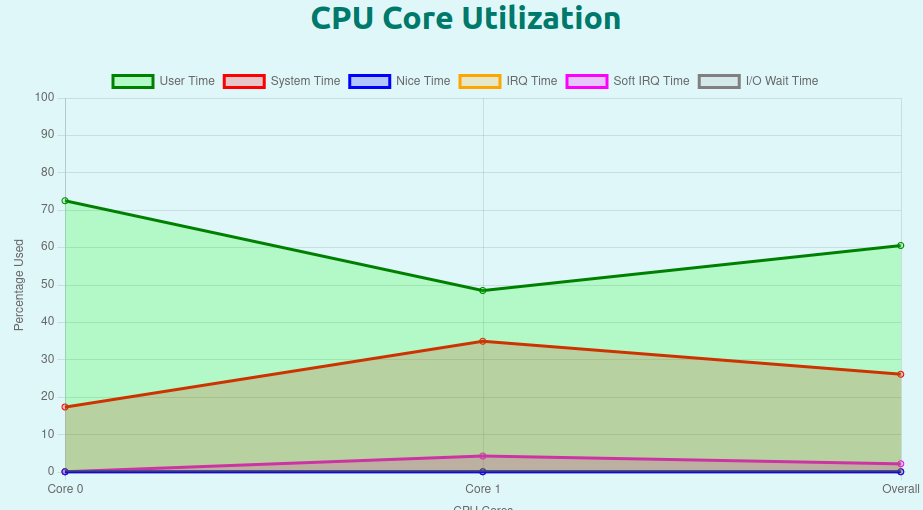
\includegraphics[width=\textwidth]{logos and images/HTOP_2.png}
    \end{minipage}
    \caption{Snapshots of the core utilizations at two different instances}
\end{figure}
The above plot updates every second, displaying the percentage of time each CPU core spends in various operational modes within a one-second interval. Additionally, the \texttt{Overall} metric represents the average CPU usage across all cores.
\subsubsection{Frontend Implementation}

Below is the implementation of the \texttt{Htop} component, written in JavaScript using React. 

\begin{minted}[fontsize=\footnotesize]{javascript}
import React, { useEffect, useState } from 'react';
import { Line } from 'react-chartjs-2';
import { Chart as ChartJS, Title, Tooltip, LineElement, PointElement, 
         CategoryScale, LinearScale, Filler } from 'chart.js';
import io from 'socket.io-client';
ChartJS.register(Title, Tooltip, LineElement, PointElement, CategoryScale, LinearScale, Filler);

const Plot4 = () => {
  const [cpuData, setCpuData] = useState([]);
  
  useEffect(() => {
    const socket = io('http://localhost:5000'); 

    socket.on('cpu_times', (data) => {
      if (Array.isArray(data) && data.length > 0) {
        setCpuData(data); 
      }
    });

    return () => {
      socket.disconnect(); 
    };
  }, []);

  const aggregateOverallData = (data) => {
    const aggregatedData = {
      user_time: 0,
      system_time: 0,
      nice_time: 0,
      irq_time: 0,
      softirq_time: 0,
      iowait_time: 0,
    };

    data.forEach(item => {
      if (item.core !== 'all') {
        aggregatedData.user_time += item.user_time || 0;
        aggregatedData.system_time += item.system_time || 0;
        aggregatedData.nice_time += item.nice_time || 0;
        aggregatedData.irq_time += item.irq_time || 0;
        aggregatedData.softirq_time += item.softirq_time || 0;
        aggregatedData.iowait_time += item.iowait_time || 0;
      }
    });

    return aggregatedData;
  };

  const generateChartData = () => {
    if (cpuData.length === 0) {
      return {}; 
    }

    const overallData = aggregateOverallData(cpuData);
    const labels = cpuData.map(item => (item.core === 'all' ? 'Overall' : Core ${item.core}));

    const chartData = {
      labels: labels,
      datasets: [
        {
          label: 'User Time',
          data: [...cpuData.map(item => item.user_time || 0), overallData.user_time],
          borderColor: 'green',
          backgroundColor: 'rgba(0, 255, 0, 0.2)',
          fill: true,
        },
        
      ],
    };

    return chartData;
  };

  const chartOptions = {
    responsive: true,
    scales: {
      x: { title: { display: true, text: 'CPU Cores' } },
      y: { 
        title: { display: true, text: 'Percentage Used' },
        beginAtZero: true,
        max: 100,
      },
    },
  };

  return (
    <div>
      <h1>Per CORE Usage</h1>
      {cpuData.length === 0 ? (
        <p>Loading data...</p>
      ) : (
        <Line data={generateChartData()} options={chartOptions} />
      )}
    </div>
  );
};

export default Plot4;
\end{minted}
\textbf{Explanation of the Code:}

1. \textbf{Dependencies and Imports:}
   The code imports the necessary dependencies for the frontend:
   \begin{itemize}
       \item \texttt{react-chartjs-2}: A React wrapper for Chart.js.
       \item \texttt{socket.io-client}: For real-time communication with the backend.
       \item \texttt{chart.js} modules: To register and configure chart components.
   \end{itemize}

2. \textbf{State Management:}
   \begin{itemize}
       \item \texttt{useState}: Manages the \texttt{cpuData} array, which stores real-time CPU usage.
       \item \texttt{useEffect}: Establishes a WebSocket connection and listens for data updates.
   \end{itemize}

3. \textbf{Data Aggregation:}
   The \texttt{aggregateOverallData} function computes the total CPU times across all cores, ignoring any data labeled as "Overall" to avoid double counting.

4. \textbf{Chart Generation:}
   The \texttt{generateChartData} function prepares data for the chart, including:
   \begin{itemize}
       \item Labels for each core and an "Overall" label.
       \item Datasets for various CPU times, such as user time, system time, and IRQ time.
   \end{itemize}

5. \textbf{Chart Options:}
   Customizes the chart's appearance:
   \begin{itemize}
       \item Labels the x-axis as "CPU Cores."
       \item Configures the y-axis to start at 0 and cap at 100 to represent percentages.
   \end{itemize}

6. \textbf{Rendering:}
   Displays a loading message until data is available. Once data is received, it renders a line chart showing per-core CPU usage.

\subsubsection{Backend Implementation}
\begin{minted}{python}
    def get_core_times():
    global cpu_times_info
    num_cores = psutil.cpu_count(logical=False)
    per_core_cpu_times = None
    while True:
        prev_per_core_cpu_times = per_core_cpu_times
        try:
            per_core_cpu_times = psutil.cpu_times(percpu=True)
        except Exception as e:
            print(f"Error getting per-core CPU times: {e}")
            continue
        
        if prev_per_core_cpu_times is not None:
            user_all, system_all, nice_all, irq_all, softirq_all, iowait_all, steal_all 
            = 0, 0, 0, 0, 0, 0, 0 
            for i, cpu_time in enumerate(per_core_cpu_times):
                cpu_times_info.append({
                    'core': i,
                    'user_time':
                    (cpu_time.user - prev_per_core_cpu_times[i].user)*100,
                    'system_time': 
                    (cpu_time.system - prev_per_core_cpu_times[i].system)*100,
                    'nice_time': 
                    (cpu_time.nice - prev_per_core_cpu_times[i].nice)*100,
                    'irq_time': (cpu_time.irq - prev_per_core_cpu_times[i].irq)*100,
                    'softirq_time': 
                    (cpu_time.softirq - prev_per_core_cpu_times[i].softirq)*100,
                    'iowait_time': 
                    (cpu_time.iowait - prev_per_core_cpu_times[i].iowait)*100,
                    'steal_time': 
                    (cpu_time.steal - prev_per_core_cpu_times[i].steal)*100,
                })
                user_all += cpu_times_info[-1]['user_time']
                system_all += cpu_times_info[-1]['system_time']
                nice_all += cpu_times_info[-1]['nice_time']
                irq_all += cpu_times_info[-1]['irq_time']
                softirq_all += cpu_times_info[-1]['softirq_time']
                iowait_all += cpu_times_info[-1]['iowait_time']
                steal_all += cpu_times_info[-1]['steal_time']
            cpu_times_info.append({
                'core': 'all',
                'user_time': (user_all/num_cores),
                'system_time': (system_all/num_cores),
                'nice_time': (nice_all/num_cores),
                'irq_time': (irq_all/num_cores),
                'softirq_time': (softirq_all/num_cores),
                'iowait_time': (iowait_all/num_cores),
                'steal_time': (steal_all/num_cores),
            })
       
        socketio.emit('cpu_times', cpu_times_info)
        time.sleep(SLEEP_INTERVAL)
        cpu_times_info = []
\end{minted}
 \begin{itemize}
        \item \texttt{PURPOSE:}
        \begin{itemize}
            \item The function captures per-core CPU times using the \texttt{psutil} library, calculates the difference in CPU times between consecutive measurements, aggregates total times across all cores, and sends the data to a client through a \texttt{Socket.IO} event. This process repeats in a loop with a delay defined by \texttt{SLEEP\_INTERVAL}.
        \end{itemize}

        \item \texttt{KEY\_VARIABLES:}
        \begin{itemize}
            \item \textbf{\texttt{cpu\_times\_info}}: A global variable used to store CPU time information for each core and the aggregated data for all cores.
            \item \textbf{\texttt{per\_core\_cpu\_times}}: Stores the most recent CPU times for all cores.
            \item \textbf{\texttt{prev\_per\_core\_cpu\_times}}: Stores the previous CPU times for all cores to calculate deltas (differences) for each time metric.
        \end{itemize}

        \item \texttt{CODE\_ANALYSIS:}
        \begin{itemize}
            \item \textbf{Global Variable Declaration:} Declares \texttt{cpu\_times\_info} as a global variable to accumulate CPU time data.
            \item \textbf{Initialization:} Initializes \texttt{per\_core\_cpu\_times} to \texttt{None} for the first iteration.
            \item \textbf{Monitoring Loop:} Continuously collects, processes, and emits CPU time data to clients.
            \item \textbf{Data Retrieval:} Retrieves per-core CPU times using \texttt{psutil.cpu\_times(percpu=True)}.
            \item \textbf{Exception Handling:} Handles any exceptions (e.g., library or system errors) to ensure the program doesn't crash and retries in the next iteration.
            \item \textbf{Skipping Invalid Iterations:} Skips processing if there are no previous CPU times to calculate differences.
            \item \textbf{Metric Totals:} Uses variables (\texttt{user\_all}, \texttt{system\_all}, \texttt{nice\_all}, \texttt{irq\_all}, \texttt{softirq\_all}, \texttt{iowait\_all}, \texttt{steal\_all}) to store total values across all cores for each CPU time metric.
            \item \textbf{Delta Calculation:} Iterates through each core's CPU times and calculates the difference (delta) for each CPU time metric by subtracting the previous values from the current ones.
            \item \textbf{Data Aggregation:} Appends the data as a dictionary to \texttt{cpu\_times\_info}.
            \item \textbf{Summary Entry:} Adds an entry to \texttt{cpu\_times\_info} representing the aggregated data across all cores.
            \item \textbf{Data Emission:} Sends the \texttt{cpu\_times\_info} list to the connected client using \texttt{Socket.IO}.
        \end{itemize}
    \end{itemize}
\subsubsection{Data used for the plot}

The JSON data sent to the frontend provides detailed CPU usage statistics for individual cores as well as aggregated metrics across all cores. Each entry in the JSON array corresponds to a specific CPU core or an "all cores" summary and contains the following fields:

\begin{itemize}
    \item \textbf{\texttt{core}}:  
    Indicates the core number (e.g., \texttt{0}, \texttt{1}, \texttt{2}, ...) or \texttt{"all"} for aggregated data across all cores. This field helps distinguish whether the data pertains to a specific core or the overall system.

    \item \textbf{\texttt{user\_time}}:  
    Represents the amount of time the CPU spent executing user-level processes (non-kernel code). This includes the execution of applications and user processes, excluding kernel/system activities.

    \item \textbf{\texttt{system\_time}}:  
    Represents the amount of time the CPU spent executing system-level processes (kernel code). This is typically used for tasks like handling I/O operations or managing system resources.

    \item \textbf{\texttt{nice\_time}}:  
    Indicates the time spent running user-level processes with a "nice" priority. Nice values are used to prioritize processes with lower importance.

    \item \textbf{\texttt{irq\_time}}:  
    Represents the time spent handling hardware interrupts. These are signals from hardware components (e.g., keyboards, network cards) that require immediate attention from the CPU.

    \item \textbf{\texttt{softirq\_time}}:  
    Indicates the time spent handling software interrupts. These are deferred tasks scheduled by the system to be handled later, often triggered by hardware interrupts.

    \item \textbf{\texttt{iowait\_time}}:  
    Represents the time the CPU spent waiting for I/O operations (e.g., disk or network) to complete. High values here may indicate I/O bottlenecks in the system.

    \item \textbf{\texttt{steal\_time}}:  
    Indicates the time that the virtual CPU was waiting for the physical CPU to become available (e.g., in virtualized environments). This is relevant in setups using virtual machines or containers.
\end{itemize}
\subsubsection{Challenges faced}
    \begin{itemize}
    \item \textbf{Calculation of times per sec}: As the /proc and psutil library both provide the user, kernel, etc times per core from the start of system, it was needed to calculate the difference for the for each second by storing the values of previous second. This resulted in a bit of overhead due to the calculation and storage.
    \item \textbf{Real-time Data Handling and Aggregation}: Ensuring smooth updates with socket connections, preventing race conditions during state updates, and handling data inconsistencies for accurate "Overall" calculations.
    \item \textbf{Dynamic Chart Updates and Configuration}: Managing efficient re-renders to avoid performance issues with large datasets, while ensuring visual clarity when displaying multiple datasets on the same chart.
\end{itemize}

\subsubsection{Uses of the plot}
\begin{itemize}
    \item \textbf{Monitoring CPU Load:} It provides a real-time visual representation of how each core's CPU time is distributed across different states (such as user time, system time, idle time, etc.) on a per-second basis. This can be used to monitor the load on each individual core in a multi-core processor.
    \item \textbf{Comparing Cores:} The plot allows for a comparison of CPU usage across different cores. This can help in identifying imbalance in workload distribution between cores, which might point to issues in parallel processing or multi-threading.
    \item \textbf{System Health Monitoring:} The \texttt{Overall} metric offers a summary of the aggregate CPU usage, which can be used to assess the general health of the system. High CPU usage across all cores may indicate that the system is under heavy load or experiencing performance issues.
    \item \textbf{Real-Time Feedback:} The plot provides real-time feedback on the system's CPU behavior, enabling users to take immediate corrective actions, such as terminating resource-heavy processes or redistributing tasks across different cores.
\end{itemize}
\subsection{Dynamic Core Migration}
\subsubsection{Frontend Implementation}

This is a simple model to visualize process migration. Process migration is modelled in the following way:
\begin{enumerate}
    \item Process are shown as discs having unique colors and names written on them.
    \item The cpu cores are shown as containers.
    \item A pipeline is shown through which a process is migrated to a different core (Analogous to how operating systems migrate processes from one core to another).
\end{enumerate}
\begin{figure}[H]
    \centering
    \begin{minipage}{0.45\textwidth}
        \centering
        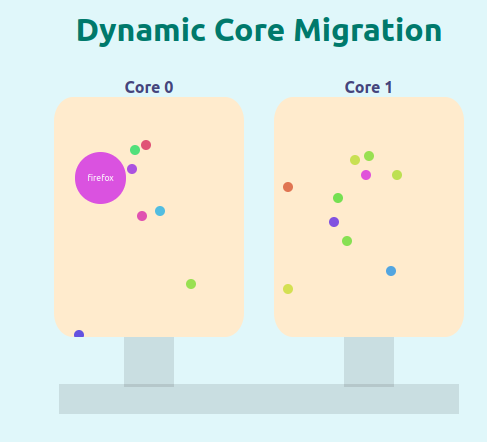
\includegraphics[width=\textwidth]{logos and images/MIG_1.png}
    \end{minipage}
    \hfill
    \begin{minipage}{0.45\textwidth}
        \centering
        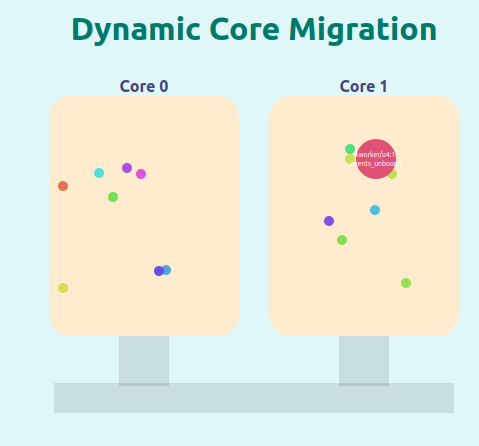
\includegraphics[width=\textwidth]{logos and images/MIG_2.png}
    \end{minipage}
    \caption{Core Migration at different time instances}
\end{figure}
The structure for creation of the model include the following:
\begin{enumerate}
    \item Data structures to store the processes and animations.
    \begin{minted}{javascript}
        const [processes, setProcesses] = useState({});
        const [processOrder, setProcessOrder] = useState([]); 
        const [processColors, setProcessColors] = useState({});
        const [animations, setAnimations] = useState({});
        const [staticPositions, setStaticPositions] = useState({});
    \end{minted}
    \item Extracting data sent through the socket connection and setting up the required data structures. 
\begin{minted}{javascript}
useEffect(() => {
    const socket = socketIOClient(SOCKET_URL);

    socket.on("cpu_migrations", (data) => {
      setProcesses((prev) => {
        const updatedProcesses = { ...prev };

        data.forEach((process) => {
          const { pid, to_core, cpu_percent, name } = process;
          const prevProcess = updatedProcesses[pid];

          if (prevProcess && prevProcess.core !== to_core) {
            setAnimations((prevAnimations) => ({
              ...prevAnimations,
              [pid]: {
                fromCore: prevProcess.core,
                toCore: to_core,
              },
            }));

            
            setTimeout(() => {
              setProcesses((finalProcesses) => ({
                ...finalProcesses,
                [pid]: {
                  ...finalProcesses[pid],
                  core: to_core,
                },
              }));
              setAnimations((prev) => {
                const updated = { ...prev };
                delete updated[pid];
                return updated;
              });
            }, 800); 
          } else {
            updatedProcesses[pid] = {
              ...prevProcess,
              pid,
              core: to_core,
              cpu_percent,
              name,
            };

            setProcessOrder((prevOrder) => {
              if (!prevOrder.includes(pid)) {
                return [...prevOrder, pid];
              }
              return prevOrder;
            });
          }
        });

        pruneOldProcesses(updatedProcesses);
        return updatedProcesses;
      });
    });

    return () => socket.disconnect();
  }, []);
\end{minted}
Functions used :
\begin{enumerate}
    \item \textbf{\texttt{useEffect}} : It is used to perform side effects in react code when some information is updated.
    \item \textbf{\texttt{socketIOClient}} : It is used to establish a connection between the frontend and the backend.
    \item \textbf{\texttt{setProcesses}} : It is used to update the processes in the state.
    \item \textbf{\texttt{setAnimations}} : It is used to update the animations in the state.
    \item \textbf{\texttt{setProcessOrder}} : It is used to update the order of the processes in the state.
    \item \textbf{\texttt{pruneOldProcesses}} : It is used to remove the old processes from the state. (It is implemented to make visualization better with lesser number of processes.)
    \item \textbf{\texttt{setTimeout}} : It is used to delay the execution of a function.
\end{enumerate}
\item Creating the model using the data structures.
\begin{minted}{javascript}
    {cores.map((core) => (
  <div key={core} className="core-with-connection">
    <div className="vertical-connection"></div>
    <div className="container">
      {[
        ...Object.values(processes)
          .filter((p) => animations[p.pid]?.fromCore === core)
          .map((p) => {
            const radius = Math.sqrt(p.cpu_percent || 1) * 10;
            return (
              <div
                key={`${p.pid}-down`}
                className="process-disc move-down"
                style={{
                  backgroundColor: getProcessColor(p.pid), 
                  width: `${radius}px`, height: `${radius}px`,
                  fontSize: `${radius / 6}px`,
                }}
              >
                {radius > 20 ? p.name : ""}
              </div>
            );
          }),

        
        ...Object.values(processes)
          .filter(
            (p) =>
              (p.core === core || animations[p.pid]?.toCore === core) &&
              !animations[p.pid] 
          )
          .map((p) => {
            const radius = Math.sqrt(p.cpu_percent || 1) * 10;
            const pos = getStaticPosition(p.pid, radius);
            return (
              <div
                key={p.pid}
                className="process-disc"
                style={{
                  backgroundColor: getProcessColor(p.pid), 
                  width: `${radius}px`, height: `${radius}px`, 
                  top: `${pos.top}px`, left: `${pos.left}px`, 
                  fontSize: `${radius / 6}px`, 
                }}
              >
                {radius > 20 ? p.name : ""} {/* Show name if large */}
              </div>
            );
          }),

        
        ...Object.values(processes)
          .filter((p) => animations[p.pid]?.toCore === core)
          .map((p) => {
            const radius = Math.sqrt(p.cpu_percent || 1) * 10;
            return (
              <div
                key={`${p.pid}-up`}
                className="process-disc move-up"
                style={{
                  backgroundColor: getProcessColor(p.pid), 
                  width: `${radius}px`, height: `${radius}px`, 
                  fontSize: `${radius / 6}px`, 
                }}
              >
                {radius > 20 ? p.name : ""} {/* Show name if large */}
              </div>
            );
          }),
      ]}
    </div>
  </div>
))}

\end{minted}
\end{enumerate}
\subsubsection{Backend Implementation}
\begin{minted}{python}
    def track_cpu_migrations():
    global core_affinity_state, migration_data

    while True:
        try:
            for proc in psutil.process_iter(['pid', 'name','cpu_percent']):
                pid = proc.info['pid']
                name = proc.info['name']
                cpu_percent=proc.info['cpu_percent']
                try:
                    
                    with open(f"/proc/{pid}/stat", "r") as stat_file:
                        stat_data = stat_file.read().split()
                        current_cpu = int(stat_data[38]) 
                except (FileNotFoundError, psutil.AccessDenied, IndexError):
                   
                    continue
                except psutil.NoSuchProcess:
                    
                    if pid in core_affinity_state:
                        del core_affinity_state[pid]
                    continue

                
                if pid in core_affinity_state:
                    previous_cpu = core_affinity_state[pid]
                    if previous_cpu != current_cpu:
                       
                        migration_entry = {
                            'pid': pid,
                            'name': name,
                            'cpu_percent': cpu_percent,
                            'from_core': previous_cpu,
                            'to_core': current_cpu,
                        }
                        migration_data.append(migration_entry)

                
                core_affinity_state[pid] = current_cpu

        except Exception as e:
            print(f"Error tracking CPU migrations: {e}")
        socketio.emit('cpu_migrations', migration_data) 
        time.sleep(SLEEP_INTERVAL) 
        migration_data=[]
\end{minted}
\begin{itemize}
    \item \texttt{PURPOSE:}
    \begin{itemize}
        \item The function continuously monitors active processes to detect migrations between CPU cores. 
        \item It tracks the core affinity for each process, identifies changes in the core a process is running on, logs migration data, and emits this information to connected clients through a Socket.IO event.
    \end{itemize}
    \item \texttt{KEY VARIABLES:}
    \begin{itemize}
        \item \textbf{\texttt{core\_affinity\_state}}: A global dictionary that tracks the last known CPU core for each process by its PID.
        \item \textbf{\texttt{migration\_data}}:  A global list that logs details of processes that have migrated between CPU cores.
        \item \textbf{\texttt{current\_cpu}}: The current CPU core a process is running on, retrieved from the /proc/[pid]/stat file.
        \item \textbf{\texttt{previous\_cpu}}:The last recorded CPU core for a process, used to detect migrations.
    \end{itemize}
    \item \texttt{CODE ANALYSIS:}
    \begin{itemize}
        \item \textbf{\texttt{Continuous Monitoring}}:
        \begin{itemize}
              \item Runs an infinite loop to track CPU core migrations without interruptions.
        \end{itemize}
       \item \textbf{\texttt{Retrieve Process Information}}:
       \begin{itemize}
            \item Iterates through all active processes using psutil.process\_iter to fetch attributes like pid, name, and cpu\_percent.
            \item Reads the /proc/[pid]/stat file to identify the current CPU core for each process.
            \item Handles exceptions like FileNotFoundError, psutil.AccessDenied, and psutil.NoSuchProcess to ensure robustness.
       \end{itemize}
        \item \textbf{\texttt{Detect and Log Migrations}}:
        \begin{itemize}
            \item Compare the current CPU core (current\_cpu) with the last recorded core (previous\_cpu) for each process.
            \item If a migration is detected, append a dictionary with migration details (pid, name, cpu\_percent, from\_core, to\_core) to migration\_data.
        \end{itemize}
\item \textbf{\texttt{Emit Migration Data}}:
\begin{itemize}
          \item Sends the logged migration data to connected clients via a Socket.IO event named cpu\_migrations.
          \item Clears migration\_data after each emission to reset for the next iteration.
\end{itemize}
    \end{itemize}
\end{itemize}   
\subsubsection{Data used for the plot}
The JSON data sent to the frontend provides information of CPU migrations of different processes occurred in a second.
\begin{itemize}
  \item \textbf{\texttt{pid}}: Identifies the specific process that has migrated. Each migration event corresponds to a unique process ID.
  \item \textbf{\texttt{name}}:Describes the name of the process. This helps to identify which process is moving between CPU cores.
  \item \textbf{\texttt{cpu\_percent}}:Shows the percentage of CPU resources being used by the process at the time of migration. This gives an indication of how much processing power the process is utilizing when the migration occurs.
  \item \textbf{\texttt{from\_core}}:Indicates the CPU core the process was previously running on. It helps track which CPU core the process migrated from.
  \item \textbf{\texttt{to\_core}}:Specifies the new CPU core the process is now running on after migration. This is crucial for identifying the migration path.
\end{itemize}
\subsubsection{Challenges faced}
\begin{enumerate}
    \item \textbf{\texttt{Real-time Data Transmission}}: Hundreds of processes are active simultaneously, and tracking their migrations in real-time can lead to high CPU usage. To prevent this, we implemented a sleep interval to reduce the frequency of data transmission.
    \item \textbf{\texttt{Data Consistency}}: Due to this sleep interval, there is a possibility of missing migrations. For this, we assume the process once sent to a core remain in the core till it is migrated to a new core. This assumption helps in maintaining the consistency of the data.
    \item \textbf{\texttt{Showing the migration path}}: We faced a challenge in showing the migration path of the processes. We used a pipeline to show the migration path of the processes.
    \item \textbf{\texttt{Showing Process Discs}}: As mentioned, we can have a lot of processes running simultaneously. We faced a challenge of showing all the processes clearly. Hence we removed the old entries for showing the latest information.
\end{enumerate}
\subsubsection{Uses of the plot}
\begin{itemize}
    \item \textbf{\texttt{Performance monitoring}}:
      \begin{itemize}
          \item Tracks process migrations across cores, highlighting CPU utilization trends.
          \item Helps identify over-utilized or under-utilized cores, ensuring optimal resource distribution.
      \end{itemize}
    \item \textbf{\texttt{Process Behavior Analysis}}:
      \begin{itemize}
          \item Visualizes processes frequently migrating between cores, revealing system optimizations or inefficiencies.
          \item Helps analyze the impact of CPU affinity on process performance.
      \end{itemize}
      \item \textbf{\texttt{System Load Analysis}}:
      \begin{itemize}
          \item Helps evaluate system behavior under different load conditions.
          \item Shows how system adapts to resource demands and manages core utilization.
      \end{itemize}
  \end{itemize}
\subsection{Dynamic 'Process-State' Tracking}
\begin{figure}[H]
    \centering
    \begin{minipage}{0.45\textwidth}
        \centering
        \includegraphics[width=\textwidth]{logos and images/GANTT_1.png}
    \end{minipage}
    \hfill
    \begin{minipage}{0.45\textwidth}
        \centering
        \includegraphics[width=\textwidth]{logos and images/GANTT_2.png}
    \end{minipage}
    \caption{Plot at different time instances}
\end{figure}

 The plot shows the state changes of each process over time as vertical segments. Each process is represented on the x-axis, and its state transitions (running, sleeping, or idle) are shown as colored segments along the y-axis. The height of each segment represents the duration of the state, allowing you to observe how a process's behavior changes over the given time range. This layout highlights time distribution across multiple processes.

\subsubsection{Frontend Implementation}
\begin{minted}{javascript}
import React, { useEffect, useState } from 'react';
import { BarChart, Bar, XAxis, YAxis, CartesianGrid, Tooltip } from 'recharts';
import io from 'socket.io-client';

const socket = io('http://127.0.0.1:5000');

function Plot5() {
  const [processStates, setProcessStates] = useState({});

  const stateColors = {
    running: '#4caf50',
    sleeping: '#FF0000',
    idle: '#FFFF00',
    default: '#8884d8',
  };

  useEffect(() => {
    socket.on('process_states', (data) => {
      setProcessStates(data);
    });

    return () => {
      socket.off('process_states');
    };
  }, []);

  const transformedData = Object.entries(processStates).map(
  ([pid, process]) => {
    const dataEntry = { name: `${process.name}` };

    process.states.forEach((state, index) => {
      const key = `${state.state}_${index}_pid${pid}`;
      dataEntry[key] = state.duration;
    });

    return dataEntry;
  });

  const allStateKeys = Array.from(
    new Set(transformedData.flatMap(data => Object.keys(data).filter(
    key => key !== 'name')))
  );

  return (
    <div className="processes">
      <h2>Process State Visualization</h2>

      <div className="legend">
        {Object.entries(stateColors).map(([state, color]) => (
          <span key={state} style={{ color, marginRight: '10px' }}>
            ● {state}
          </span>
        ))}
      </div>

      {transformedData.length > 0 ? (
        <BarChart
          width={600}
          height={400}
          data={transformedData}
          margin={{
            top: 5,
            right: 30,
            left: 20,
            bottom: 60,
          }}
        >
          <CartesianGrid strokeDasharray="3 3" />
          <XAxis dataKey="name" 
            angle={-45}
            textAnchor='end'
          />
          <YAxis domain={[0, 'auto']} />
          <Tooltip />

          {allStateKeys.map((key) => {
            const stateType = key.split('_')[0];
            return (
              <Bar
                key={key}
                dataKey={key}
                stackId="a"
                fill={stateColors[stateType] || stateColors.default}
                barSize={20}
              />
            );
          })}
        </BarChart>
      ) : (
        <p>No data available to display.</p>
      )}
    </div>
  );
}

export default Plot5;

\end{minted}
\subsubsection{Backend Implementation}

\begin{minted}{python}
process_states = {}  
TIME_RANGE = 1  
SLEEP_INTERVAL1 = 0.1  
def monitor_process_states():
    global process_states, TIME_RANGE
    last_emit_time = time.time()  

    while True:
        current_time = time.time() 
        start_time = current_time - TIME_RANGE  
        for proc in psutil.process_iter(attrs=['pid', 'name', 'status',
        'cpu_percent']):
            try:
                pid = proc.info['pid']
                state = proc.info['status']
                cpu_usage = proc.info['cpu_percent']

                if pid not in process_states:
                    process_states[pid] = {
                        'name': proc.info['name'],
                        'states': []
                    }

                states = process_states[pid]['states']
                current_time_s = time.time()
                if states :
                 states[-1]['end_time'] = current_time_s
                 states[-1]['duration'] = states[-1]['end_time'] -
                 states[-1]['start_time']
                if states and states[-1]['state'] == state:
                    pass
                else:

                    
                    states.append({
                        'state': state,
                        'start_time': current_time_s,
                        'end_time': current_time_s,
                        'duration': 0  
                    })
                process_states[pid]['states'] = [
                    state for state in process_states[pid]['states']
                    if state['end_time'] > start_time  
                ]
                    
            except (psutil.NoSuchProcess, psutil.AccessDenied):
                continue

        emit_process_states = {}
        if time.time() - last_emit_time >= 2:
            for pid, data in process_states.items():
                total_duration = 0
                adjusted_states = []

                for state in data['states']:
                    duration = min(state['end_time'], start_time + TIME_RANGE) - max(state['start_time'], start_time)

                    if duration > 0:
                        total_duration += duration
                        adjusted_states.append({
                            'state': state['state'],
                            'start_time': max(state['start_time'], start_time),
                            'end_time': min(state['end_time']
                            , start_time + TIME_RANGE),
                            'duration': duration
                        })
                                
                emit_process_states[pid] = {
                    'name': data['name'],
                    'states': adjusted_states
                }

            running_processes = {
             pid: data for pid, data in emit_process_states.items()
             if any('running' in state['state'] for state in data['states'])
             }   


            
            socketio.emit('process_states', running_processes)  
            last_emit_time = time.time() 

        time.sleep(SLEEP_INTERVAL1)  


\end{minted}

\subsubsection{Data used for the plot}
The data for the plot is derived from the \texttt{process\_states} dictionary, which tracks process activities over a sliding window of the last \texttt{TIME\_RANGE} seconds. This dictionary is structured to record details for each process, identified by its unique PID and name. 

For each process, a list of state intervals is maintained. Each state interval comprises:
\begin{itemize}
    \item \textbf{State:} Represents the current activity of the process, such as \textit{running}, \textit{sleeping}, or \textit{idle}.
    \item \textbf{Start Time:} The timestamp when the process entered this state.
    \item \textbf{End Time:} The timestamp when the process exited this state, or the current time if it is ongoing.
    \item \textbf{Duration:} The time the process spent in the specific state, computed as the difference between \texttt{end\_time} and \texttt{start\_time}.
\end{itemize}


\subsubsection{Challenges faced}

During the development and implementation of the plot and process monitoring system, several challenges were encountered:

\begin{itemize}
     \item \textbf{Memory Management:} With the continuous monitoring of multiple processes, memory management became a significant challenge. The \texttt{process\_states} dictionary, which stores state intervals for each process, could potentially grow large over time, especially when monitoring long-running processes. To avoid excessive memory consumption, it was crucial to implement an efficient data structure and clean-up mechanism. State data for processes that no longer exist or whose state transitions have moved outside the defined time window needed to be regularly purged. Additionally, implementing proper memory management practices like limiting the depth of stored state intervals, discarding old data, and ensuring that only relevant state transitions are kept helped to optimize memory usage. These strategies ensured that the system remained responsive and stable without excessive memory overhead.

     \item \textbf{Missing Running Intervals:} One of the challenges encountered during the monitoring process was the issue of missing running intervals, particularly when the sampling interval (sleeping interval) was set to 1 second and the time range was set to 10 seconds. Since the process states were being updated at a fixed 1-second interval, there was a possibility that a running process could transition between the sampled states without being captured in the recorded data. This resulted in a gap where the running interval was either missed entirely or inaccurately represented. This issue was noticed because we didn't even get any running processes initially because of our sleeping interval(1 sec) . But after keeping the interval for 0.01 second we are able detect those running processes .

     Even after keeping the interval for 0.01 second we still faced an issue with the number of process . As the number is too high we got very thin lines on x axis and unable to notice the processes separately , so we filtered the \texttt{process\_states} to store only the processes which have non zero duration of running state in our considered \textbf{Time Range} .

     \item \textbf{Color Representation and Clarity:} Designing the plot for clarity was challenging, especially when processes rapidly switched between states. The need to display even small state transitions required careful attention to the chart's design, including ensuring that all states were visible while avoiding clutter.
\end{itemize}

\subsubsection{Uses of the plot}
The plot provides a visual representation of process states over time, making it useful in several ways. It helps in understanding the behavior and resource utilization of processes, such as identifying how long each process spends in different states (running, sleeping, idle). By visualizing these transitions, it becomes easier to detect patterns in process activity, monitor performance, and spot potential issues like processes stuck in the sleeping state or those that are frequently idle. 

This plot can be particularly valuable for:
\begin{itemize}
    % \item \textbf{System Performance Monitoring:} It allows us to monitor the efficiency of process scheduling and CPU usage, providing insights into which processes are consuming resources at different times.
    \item \textbf{Optimization:} By observing the time spent in idle or sleeping states, it becomes possible to identify opportunities for optimization, such as reducing unnecessary wake-ups or improving the scheduling of processes or identifying the process which are in idle or sleep state for the most of the time .
    \item \textbf{Debugging and Troubleshooting:} The chart helps in identifying abnormal process behavior, such as processes frequently switching between states or processes stuck in a particular state, making it a useful tool for debugging.
\end{itemize}
Overall, the plot serves as an essential tool for monitoring and improving system performance, making it easier to track process behavior over time and make informed decisions based on real-time data.

\subsection{CFS - Process Scheduling Tree}
\begin{figure}[H]
    \centering
    \begin{minipage}{0.8\textwidth}
        \centering
        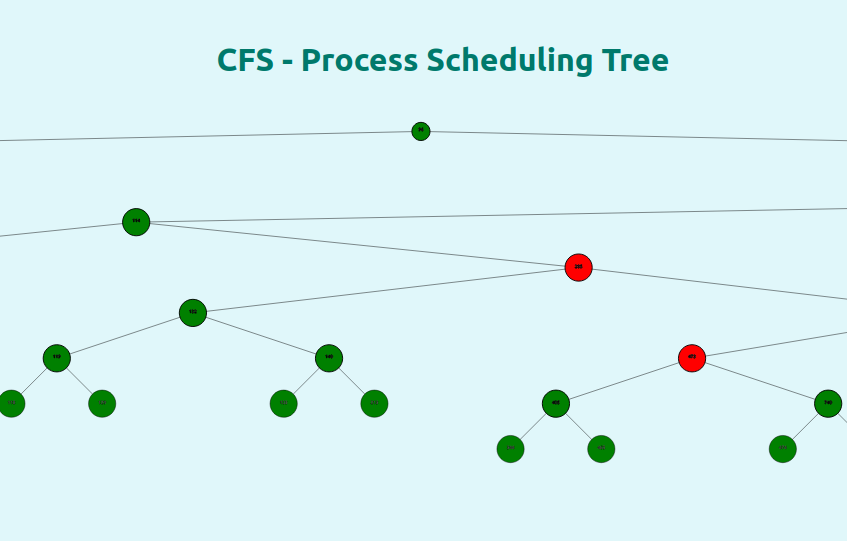
\includegraphics[width=\textwidth]{logos and images/CFS_1.png}
    \end{minipage}
    \hfill
    
    \caption{Snapshot of the Tree}
\end{figure}
The graph visualizes the Completely Fair Scheduler (CFS)'s internal management of processes as a Red-Black Tree. Each node in the tree represents a process, uniquely identified by its Process ID (PID). The nodes are organized based on their virtual runtime (\texttt{vruntime}), which determines the priority of processes in the scheduling system.
\subsubsection{Frontend Implementation}
\begin{minted}{javascript}
import React, { useEffect, useState } from "react";
import { io } from "socket.io-client";
import Tree from "react-d3-tree";

const Plot6 = () => {
  const [treeData, setTreeData] = useState(null);

  useEffect(() => {
    const socket = io("http://localhost:5000");

    socket.on("tree_data", (data) => {
      if (data && data.root) {
        setTreeData(formatTreeData(data.root));
      }
    });

    return () => {
      socket.disconnect();
    };
  }, []);

  const formatTreeData = (node) => {
    if (!node) return null;
    return {
      name: `${node.pid}`,
      attributes: {},
      children: [formatTreeData(node.left), formatTreeData(node.right)].filter(
        (child) => child !== null
      ),
      nodeColor: node.color === "black" ? "green" : node.color,
      nodeRadius: Math.max(10, String(node.pid).length * 10),
    };
  };

  return (
    <div
      className="processes"
      style={{
        width: "100%",
        height: "500px",
        display: "flex",
        flexDirection: "column",
        alignItems: "center",
      }}
    >
      <h1 style={{ marginBottom: "20px" }}>CFS - Process Scheduling Tree</h1>
      {treeData ? (
        <Tree
          data={treeData}
          orientation="vertical"
          pathFunc="straight"
          translate={{ x: 920, y: 30 }}
          nodeSize={{ x: 200, y: 100 }}
          renderCustomNodeElement={({ nodeDatum }) => (
            <g style={{ color: "white" }}>
              <circle
                r={nodeDatum.nodeRadius || 10}
                fill={nodeDatum.nodeColor}
              />
              <text className="node-text">{nodeDatum.name}</text>
            </g>
          )}
        />
      ) : (
        <p>Loading tree data...</p>
      )}
    </div>
  );
};

export default Plot6;

\end{minted}
\begin{itemize}
    \item \textbf{WebSocket:} Connects to a server to receive process tree data in JSON format.
    \item \textbf{Data Formatting:} Processes JSON nodes into a hierarchical structure with attributes like \texttt{name}, \texttt{color}, and \texttt{radius}.
    \item \textbf{Visualization:} Renders a vertical tree where nodes are styled as colored circles with PIDs displayed.
    \item \textbf{Styling:} The component is styled for responsive display with centered visualization.
    \item \textbf{Error Handling:} Disconnects WebSocket on unmount and shows a loading message until data is available.
\end{itemize}
\subsubsection{Backend Implementation}
\begin{minted}{python}
    class Node:
    def __init__(self, key, value, name):
        self.key = key
        self.value = value
        self.name = name
        self.color = 'red'
        self.left = None
        self.right = None
        self.parent = None

class RedBlackTree:
    def __init__(self):
        self.TNULL = Node(0, 0, "")
        self.TNULL.color = 'black'
        self.root = self.TNULL

    def insert(self, key, value, name):
        node = Node(key, value, name)
        node.parent = None
        node.left = self.TNULL
        node.right = self.TNULL
        node.color = 'red'

        parent = None
        current = self.root

        while current != self.TNULL:
            parent = current
            if node.value < current.value:
                current = current.left
            else:
                current = current.right

        node.parent = parent
        if parent is None:
            self.root = node
        elif node.value < parent.value:
            parent.left = node
        else:
            parent.right = node

        if node.parent is None:
            node.color = 'black'
            return

        if node.parent.parent is None:
            return

        self.fix_insert(node)

    def fix_insert(self, k):
        while k.parent.color == 'red':
            if k.parent == k.parent.parent.right:
                u = k.parent.parent.left
                if u.color == 'red':
                    u.color = 'black'
                    k.parent.color = 'black'
                    k.parent.parent.color = 'red'
                    k = k.parent.parent
                else:
                    if k == k.parent.left:
                        k = k.parent
                        self.right_rotate(k)
                    k.parent.color = 'black'
                    k.parent.parent.color = 'red'
                    self.left_rotate(k.parent.parent)
            else:
                u = k.parent.parent.right
                if u.color == 'red':
                    u.color = 'black'
                    k.parent.color = 'black'
                    k.parent.parent.color = 'red'
                    k = k.parent.parent
                else:
                    if k == k.parent.right:
                        k = k.parent
                        self.left_rotate(k)
                    k.parent.color = 'black'
                    k.parent.parent.color = 'red'
                    self.right_rotate(k.parent.parent)
            if k == self.root:
                break
        self.root.color = 'black'

    def left_rotate(self, x):
        y = x.right
        x.right = y.left
        if y.left != self.TNULL:
            y.left.parent = x
        y.parent = x.parent
        if x.parent is None:
            self.root = y
        elif x == x.parent.left:
            x.parent.left = y
        else:
            x.parent.right = y
        y.left = x
        x.parent = y

    def right_rotate(self, x):
        y = x.left
        x.left = y.right
        if y.right != self.TNULL:
            y.right.parent = x
        y.parent = x.parent
        if x.parent is None:
            self.root = y
        elif x == x.parent.right:
            x.parent.right = y
        else:
            x.parent.left = y
        y.right = x
        x.parent = y

    def get_root(self):
        return self.root

    def inorder_helper(self, node):
        if node != self.TNULL:
            self.inorder_helper(node.left)
            print(f"{node.key}: {node.value} ({node.name})")
            self.inorder_helper(node.right)

    def inorder(self):
        self.inorder_helper(self.root)

def serialize_tree(node, TNULL):
    if node == TNULL:
        return None
    return {
        'pid': node.key,
        'vruntime': node.value,
        'name': node.name,
        'color': node.color,
        'left': serialize_tree(node.left, TNULL),
        'right': serialize_tree(node.right, TNULL)
    }

def get_process_vtimes():
    while True:
        rbt = RedBlackTree()
        for proc in psutil.process_iter(['pid', 'name', 'cpu_times']):
            try:
                vtimes = proc.cpu_times()
                rbt.insert(proc.info['pid'], vtimes.user + vtimes.system, proc.info['name'])
            except (psutil.NoSuchProcess, psutil.AccessDenied):
                continue
        tree_data = serialize_tree(rbt.get_root(), rbt.TNULL)
        socketio.emit('tree_data', {'root': tree_data})
        time.sleep(SLEEP_INTERVAL)

\end{minted}
\begin{itemize}
    \item The \texttt{Node} class represents a single node in a red-black tree, storing attributes like \texttt{key}, \texttt{value}, \texttt{name}, and pointers to parent and child nodes.
    \item The \texttt{RedBlackTree} class manages the red-black tree, supporting insertion and ensuring tree properties through balancing methods such as \texttt{fix\_insert}, \texttt{left\_rotate}, and \texttt{right\_rotate}.
    \item The \texttt{serialize\_tree} function converts the red-black tree structure into a serializable format, enabling data exchange or visualization.
    \item The \texttt{get\_process\_vtimes} function uses \texttt{psutil} to iterate over active processes, fetch their virtual runtimes, and insert them into a red-black tree. The serialized tree is then emitted via a WebSocket using \texttt{socketio}.
    \item This implementation integrates real-time process monitoring with structured tree data representation, ensuring efficient scheduling insights.
\end{itemize}
\subsubsection{Data used for the plot}
The provided data is in JSON format and represents a hierarchical structure of processes in a system. Each process is represented as a node in a tree, with the following attributes:

\begin{itemize}
    \item \textbf{pid}: The Process ID (PID), a unique identifier for each process.
    \item \textbf{vruntime}: A value representing the runtime of the process within the scheduler, which helps determine process scheduling priority.
    \item \textbf{name}: The name or description of the process.
    \item \textbf{color}: A value that specifies the color of the node in the tree (typically black or red), often used to maintain balance in a Red-Black Tree.
    \item \textbf{left}: A pointer to the left child node, which represents the next lower-priority process in the hierarchy.
    \item \textbf{right}: A pointer to the right child node, representing the next higher-priority process.
\end{itemize}

The JSON structure is a recursive tree where each process may have child processes (left and right) represented as nested objects. The root of the tree represents the main process, and each child node (process) can further branch out into its respective child processes, forming a detailed hierarchy of processes.

\subsubsection{Challenges faced}
Will fill wait.
\subsubsection{Uses of the plot}

\begin{itemize}
    \item \textbf{Visualization of Scheduler Behavior:} 
    The CFS tree organizes processes based on their \textit{vruntime}, which reflects the amount of CPU time they have consumed relative to others. Displaying this tree helps visualize how the scheduler prioritizes processes. The project can show which processes are ``closer'' to being scheduled next, offering a clear view of scheduling fairness.

    \item \textbf{Understanding Process Prioritization:} 
    The CFS ensures fairness by scheduling the process with the smallest \textit{vruntime} first. Displaying the tree can help explain why certain processes are scheduled ahead of others and how their priorities evolve over time.

    \item \textbf{Performance Analysis and Optimization:} 
    By analyzing the CFS tree, users can identify processes with disproportionate \textit{vruntime} values, which might indicate bottlenecks or inefficiencies in resource allocation.
\end{itemize}

\end{document}